% Author: Santiago Faci <santi@arkabytes.com>
% http://github.com/sfaci/masc

\documentclass[xcolor={dvipsnames}]{beamer}
\setbeamertemplate{navigation symbols}{}

\usepackage{beamerthemeshadow}
\usepackage{hyperref}
\usepackage[spanish]{babel}
\usepackage{url}
\usepackage[utf8]{inputenc}

\definecolor{resalta}{cmyk}{0,1,0,0}

\usepackage{listings}
\lstset{basicstyle=\tiny\ttfamily,breaklines=true}
\lstset{framextopmargin=50pt}
\lstset{keywordstyle=\tiny\color{blue}\bfseries}
\lstset{stringstyle=\tiny\color{red}\ttfamily}
\lstset{commentstyle=\tiny\color{OliveGreen}\ttfamily}
\lstset{showstringspaces=false}

\begin{document}
\title{masc: malware scanner}

% logo
\titlegraphic{
\includegraphics[scale=0.2]{hacktoberfest}
}

\begin{frame}
\titlepage
\end{frame}

\begin{frame}\frametitle{Índice}\tableofcontents
\end{frame} 


\section{¿Qué es masc?}
\begin{frame}\frametitle{¿Qué es masc?}

    \begin{block}{malware web scanner}
    Escanea un sitio web ya comprometido en busca de malware con el objetivo de eliminarlo
    \end{block}

    \begin{itemize}
        \item También corrige problemas de seguridad conocidos propios de los sitios web
        \item Comportamiento a medida de algunos CMS concretos (actualmente WordPress y Drupal)
        \item Puede trabajar basándose en diccionarios que pueden ser ampliados y mejorados
        \item La idea es que sea fácilmente extensible para que se adapte a otros CMS y arquitecturas web
    \end{itemize}
\end{frame}

\section{¿Cómo funciona masc?}
\begin{frame}\frametitle{¿Cómo funciona masc? I}

    \begin{itemize}
        \item Busca y/o limpia, automáticamente, malware en un sitio web que sabemos que ha sido atacado
        \item Utiliza instalaciones limpias (que descarga si es necesario) para comparar y encontrar ficheros sospechosos
        \item Trabaja principalmente basándose en firmas y reglas YARA del proyecto OWASP \href{https://wiki.owasp.org/index.php/OWASP_Web_Malware_Scanner_Project}{WebMalwareScanner}
        \item También se integra con ClamAV (si está instalado) para que escanee el sitio en busca de virus
    \end{itemize}
\end{frame}

\section{¿Cómo funciona masc?}
\begin{frame}\frametitle{¿Cómo funciona masc? II}

    \begin{itemize}
        \item Antes de realizar una limpieza del malware del sitio realiza un backup del mismo
        \item El usuario puede restaurar ese backup previo usando la herramienta
        \item Toda la actividad de \emph{masc} queda registrada en logs
    \end{itemize}
\end{frame}

\begin{frame}\frametitle{¿Cómo funciona masc? III}

    \begin{itemize}
        \item Además limpia contenido no necesario del sitio y ejecuta algunas otras operaciones para ayudar en su protección
            \begin{itemize}
                \item Elimina todo tipo de README del core y temas (en WordPress)
                \item Evita el listado de directorios
                \item Elimina el metatag que identifica la versión (en WordPress)
                \item Corrige los permisos incorrectos de algunas carpetas
            \end{itemize}
        \item También es capaz de monitoriza el sitio web completo en busca de cambios y los registra en un log
    \end{itemize}
\end{frame}

\section{Demo}
\subsection{La herramienta}
\begin{frame}\frametitle{masc como herramienta}
    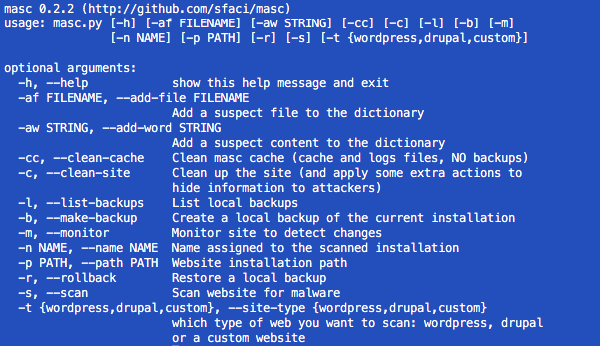
\includegraphics[scale=0.4]{options}
\end{frame}

\subsection{Ecaneo de un sitio}
\begin{frame}\frametitle{Escaneo de un sitio WordPress}
    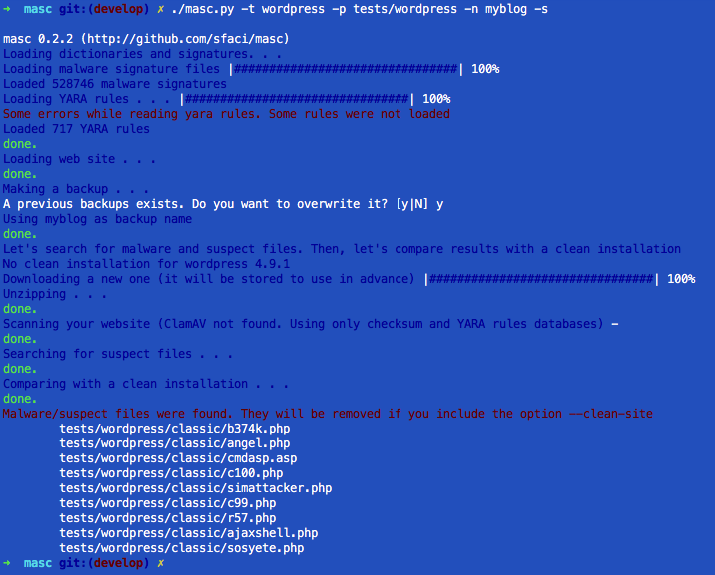
\includegraphics[scale=0.3]{wordpress_scan}
\end{frame}

\subsection{Escaneo y limpieza de un sitio}
\begin{frame}\frametitle{Escaneo y limpieza de un sitio WordPress}
    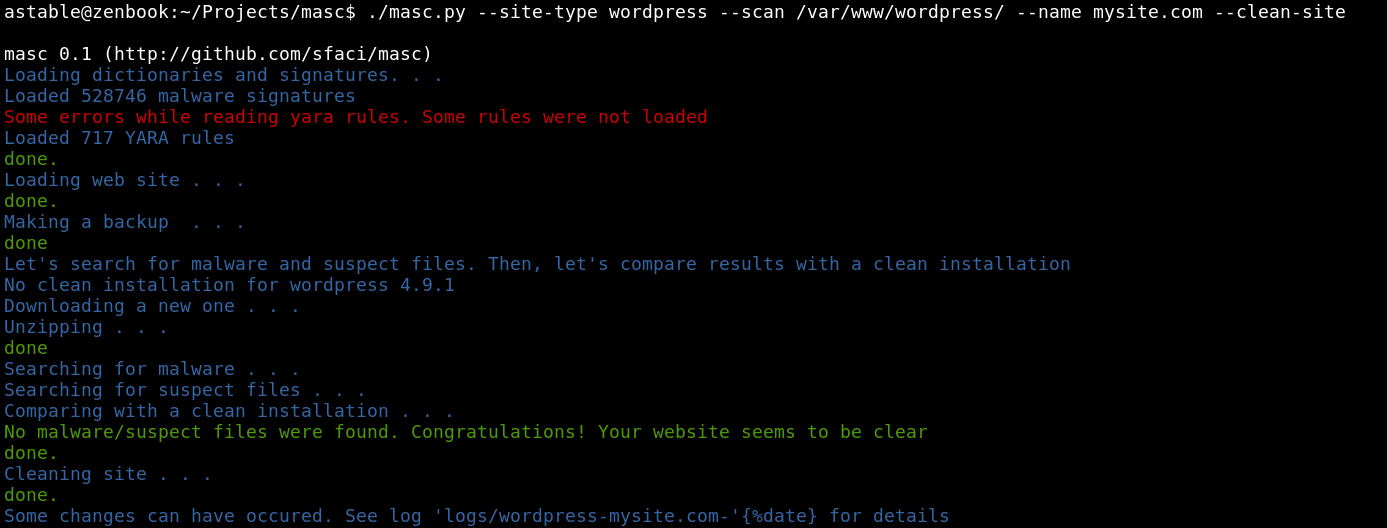
\includegraphics[scale=0.35]{complete}
\end{frame}

\subsection{Logs}
\begin{frame}\frametitle{Ficheros log}
    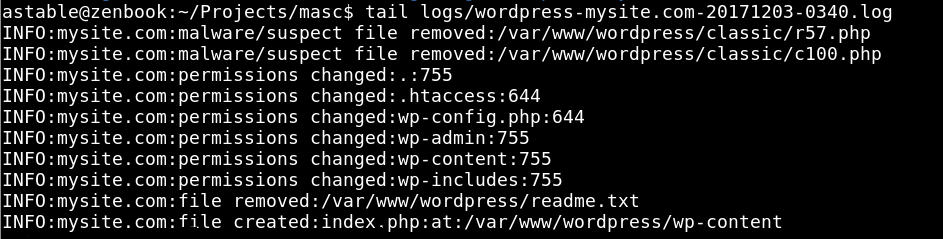
\includegraphics[scale=0.4]{log}
\end{frame}

\section{¿Cómo puede mejorar?}
\begin{frame}\frametitle{Ideas para el futuro}
    \begin{block}{Ideas para el futuro}
    \begin{itemize}
        \item Ampliar la base de datos de firmas y reglas YARA (hay repositorios online)
        \item Que sea capaz de limpiar código inyectado en ficheros legítimos
        \item Diseñar un interfaz web
        \item Escaneo remoto de sitios web
        \item Convertirlo en herramienta web como servicio en la nube
        \item Y unas cuantas más, además de otros tantos arreglos que se le pueden hacer (Ver issues del proyecto)
    \end{itemize}
    \end{block}
\end{frame}

\begin{frame}\frametitle{Fin}
    \begin{center}
        
\includegraphics[scale=0.3]{hacktoberfest}
     \end{center}
\end{frame}

\end{document}
